\documentclass[conference]{IEEEtran}
\usepackage[T1]{fontenc}
\usepackage{graphicx}
\usepackage{booktabs}
\usepackage{amsmath}
\usepackage{amsfonts}
\usepackage{cite}
\usepackage{url}
\usepackage{array}
\usepackage{multirow}

\newcommand{\etal}{et~al.\ }
\newcommand{\X}{\mathcal{X}}
\newcommand{\A}{\mathcal{A}}

\begin{document}

\title{A Longitudinal Knowledge-Graph-Aware Framework for Diabetes Progression Modelling with Temporal Attention and Calibrated Fusion}

\author{
\IEEEauthorblockN{Research Prototype Authors}
\IEEEauthorblockA{Longitudinal Diabetes Progression Research System\\
Correspondence: project repository}
}

\maketitle

\begin{abstract}
Accurately predicting the progression of chronic conditions such as
type 2 diabetes requires models that combine longitudinal clinical
measurements, population-scale similarity structures, and calibrated
uncertainty. In this paper we present a modular research framework that
integrates a patient-level knowledge graph, trajectory-derived features,
and a staged pipeline of ten learning models. We introduce three
technical components designed for longitudinal patient data: a
Temporal Attention Graph Neural Network (TAGNN) that weights
neighbour contributions by trajectory divergence through a learned
temporal gate; a Multi-Head Feature Interaction Network (MHFIN) that
explicitly models pairwise feature interactions through multiple
projection heads; and a Confidence-Calibrated Fusion (CCF) layer that
stacks base-model probabilities and learns per-model reliability
coefficients on out-of-fold predictions. A fourth component, Patient
Trajectory Clustering (PTC), augments features with shape-based
trajectory cluster identifiers. Models are evaluated on a patient-level
stratified split using accuracy, precision, recall, F1 score, area under
the ROC and PR curves, Brier score, and log loss. An ablation confirms
that adding knowledge-graph edges and longitudinal features yields
successive improvements over a plain graph model. All results are
served through a FastAPI backend and an interactive React dashboard,
making the system usable both as a research platform and as a
decision-support prototype. The system is explicitly presented as a
research and decision-support tool rather than a diagnostic device.
\end{abstract}

\begin{IEEEkeywords}
graph neural networks, knowledge graphs, longitudinal clinical data,
diabetes progression, temporal attention, model calibration, ensemble
fusion, interpretability
\end{IEEEkeywords}

\section{Introduction}

Diabetes is a progressive chronic condition whose management depends on
the ability to anticipate how an individual's metabolic state will
evolve over time \cite{ada}. Glycated haemoglobin (HbA1c), fasting
glucose, body-mass index, and blood pressure are routinely recorded at
successive clinical visits, producing a longitudinal record that is
fundamentally different from the single-snapshot data assumed by most
tabular classifiers. A model that treats each row as independent
discards the ordering of measurements and the shape of the trajectory;
a model that ignores patient-to-patient structure cannot exploit
similarity between individuals who share conditions or metabolic
patterns.

This paper describes a fully implemented research framework for
diabetes progression modelling that brings together four modelling
ideas that are normally studied in isolation: (i)~knowledge-graph
reasoning over patient and condition entities, (ii)~longitudinal
trajectory features derived from multiple visits, (iii)~graph neural
networks with attention, and (iv)~calibrated probabilistic fusion for
ensemble decisions. The framework is organised as a layered pipeline
-- data, pre-processing and knowledge, modelling, and serving -- and is
evaluated on a cohort of 240 patients with four visits each.

%----------------------------------------------------------------------
\section{Related Work}

Graph neural networks generalise deep learning to relational data by
iteratively propagating and aggregating messages over a graph
structure \cite{scarselli,kipf2017,hamilton2017}. Attention mechanisms,
originally introduced for sequence modelling \cite{vaswani}, have been
adapted to graphs to let a node decide \emph{which} neighbours should
influence its representation. However, most graph attention variants
attend over structural or feature similarity and do not explicitly
consider whether two patients are co-evolving along a clinical
trajectory. Our TAGNN closes this gap with a temporal gate that
compares the feature trajectories of the two endpoints of each edge.

Ensembles improve robustness, but naive averaging ignores the fact that
models differ in reliability. Calibration of modern neural networks was
studied by Guo~\etal\cite{guo}, who showed that confidence is often
poorly calibrated and can be corrected with a learnt temperature or
probabilistic layer. We adopt a logistic stacking layer that learns
per-model coefficients rather than a single temperature, so the fusion
weight of each model emerges directly from its out-of-fold behaviour.

Interpretability of black-box models is a recurring concern in clinical
applications. Local explanation methods such as LIME and SHAP
\cite{lime,shap} approximate per-instance feature contributions. Our
system instead surfaces interpretable artefacts directly: trajectory
features, cluster identifiers, and learned attention weights are
reported alongside every prediction in the dashboard.

Tabular ensemble methods such as random forests \cite{breiman} and
gradient boosting \cite{xgboost} remain strong baselines on structured
clinical data, and we retain them as reference points. The Pima Indians
Diabetes dataset \cite{pima} is used as the canonical public benchmark
for diabetes outcome prediction; our synthetic cohort generator is
designed to expose the same type of longitudinal structure.

%----------------------------------------------------------------------
\section{System Architecture}

The architecture is organised into four layers (Fig.~\ref{fig:arch}).
The \emph{data layer} accepts one of three sources: a reproducible
synthetic cohort generator, the public Pima Indians dataset, or an
arbitrary user-provided longitudinal CSV (by path, URL, or upload).
The \emph{pre-processing and knowledge layer} validates and
standardises the data, builds the knowledge graph, and derives
per-patient trajectory features and cluster identifiers. The
\emph{modelling layer} trains ten models: four tabular baselines, a
plain graph model and two progressive graph-kernel variants, the two
novel architectures TAGNN and MHFIN, and the CCF stacked fusion. The
\emph{serving layer} evaluates every model on the held-out patient
split, persists artefacts to JSON and PyTorch checkpoint files, and
exposes all results through a FastAPI backend and a React dashboard
served by Vite.

\begin{figure}[!t]
\centering
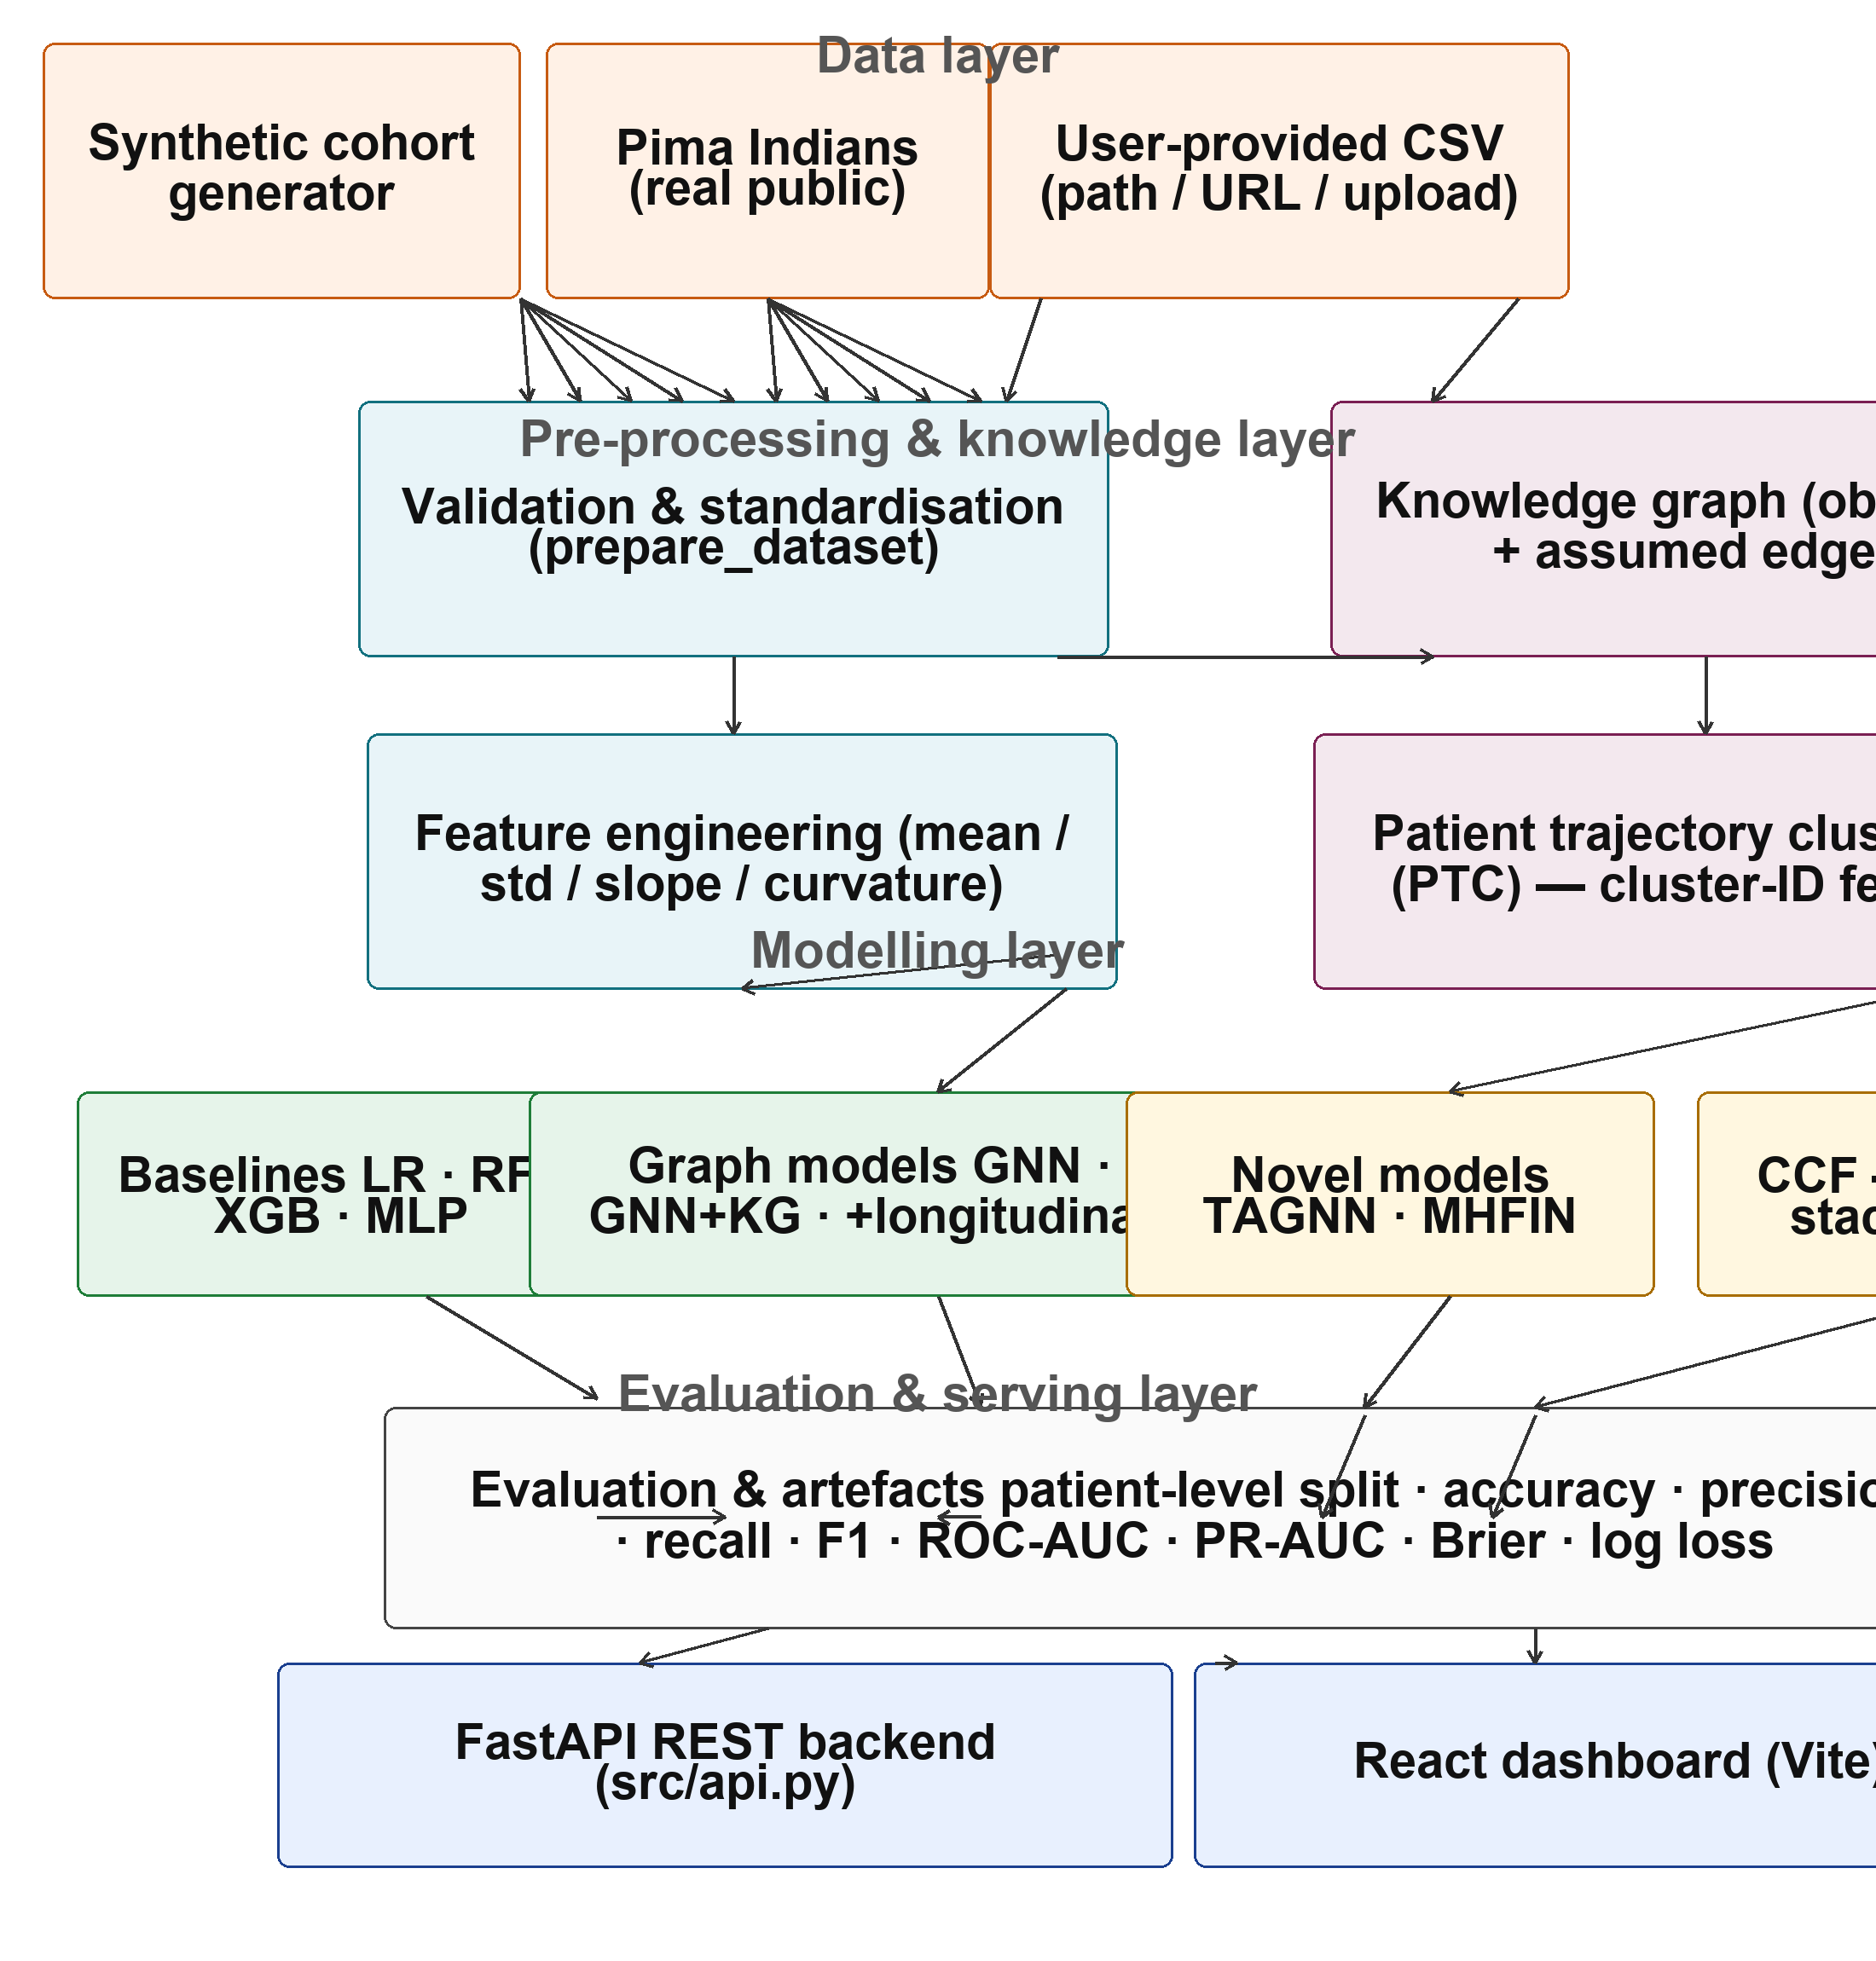
\includegraphics[width=\columnwidth]{figures/architecture.png}
\caption{Layered system architecture. Data flows from three sources
through validation, knowledge-graph construction and feature
engineering into the modelling and evaluation layers, and is served
through a REST backend and a React dashboard.}
\label{fig:arch}
\end{figure}

%----------------------------------------------------------------------
\section{Methodology}

\subsection{Data and Pre-processing}

Each patient is represented by up to four labelled visits with visit
number, date, age, HbA1c, glucose, BMI, systolic and diastolic blood
pressure, and a condition label. The progression target is derived from
the trajectory: a patient progresses if the final HbA1c exceeds the
first by at least 0.5\,\% or if the final value is at least 6.5\,\%.
Validation enforces column presence, numeric coercion, and enough
visits per patient to support longitudinal features.

\subsection{Knowledge-Graph Construction}
\label{sec:kg}

The knowledge graph is a directed multigraph with two node types:
patient nodes and condition nodes. Two edge types are distinguished:
\emph{observed} edges from a patient to their condition, justified by
the dataset, and \emph{assumed similarity} edges between patients who
share a condition, explicitly labelled as modelling assumptions rather
than causal or clinical evidence. Keeping these edge types separate is
deliberate: it lets downstream models exploit population similarity
while making the epistemic status of each edge auditable.

\subsection{Feature Engineering}

From the first three visits we compute per-feature means and standard
deviations for the six clinical measurements, then fit a linear model
over the visit index to obtain the HbA1c slope, glucose slope, and an
HbA1c curvature term. This yields a compact patient-level vector that
retains both the level and the direction of change of each measurement.

\subsection{Patient Trajectory Clustering (PTC)}

Rather than clustering patients on raw values, PTC clusters on
trajectory \emph{shape}. The HbA1c slope and, when available, the
curvature define a two- (or three-) dimensional space that is
segmented with $k$-means ($k=5$). Each patient receives a cluster
identifier that is one-hot encoded and concatenated to the feature
matrix, providing the classifiers with population-level progression
patterns.

\subsection{Baseline and Graph Models}

The tabular baselines are logistic regression, a random forest, an
XGBoost classifier, and a multilayer perceptron, all trained on the
standardised feature matrix. The graph models regress on a shared
message-passing backbone: features of neighbour nodes are aggregated
by weighted sum, normalised by degree, gated by a learned attention
signal, and passed through a two-layer head. Three configurable
variants are trained: a plain graph model, a knowledge-graph variant
whose edges encode elevated-HbA1c co-morbidity similarity, and a
longitudinal variant that additionally consumes slope and curvature
features.

\subsection{Temporal Attention GNN (TAGNN)}
\label{sec:tagnn}

TAGNN augments standard message passing with a learned temporal gate.
For each directed edge $(u,v)$, a two-layer sigmoid gate receives the
concatenation of the source and target feature vectors and produces a
scalar in $(0,1)$ that down-weights neighbours whose feature trajectory
diverges from the target patient:
\begin{equation}
m_{uv} = g\left([x_u; x_v]\right) \odot (W_N\, x_v), \qquad
g(z)=\sigma(W_2\,\mathrm{ReLU}(W_1 z+ b_1)+b_2),
\end{equation}
where $x_u$ is the feature vector of node $u$, $W_N$ is the neighbour
projection, and $g$ is the temporal gate. Messages are summed per
source node, normalised by degree, combined with the self-projection,
layernormed, and passed through a ReLU. The model stacks two such
layers followed by a linear classification head, and is trained with
the binary cross-entropy loss over the training-patient mask with an
Adam optimiser.

\subsection{Multi-Head Feature Interaction Network (MHFIN)}

MHFIN enriches the base representation with explicitly modelled
pairwise feature interactions. A set of $k$ linear projections (here
$k=4$) maps the input to $k$ low-dimensional embeddings; the original
features and all projections are concatenated into a single enriched
vector that feeds a two-layer classification head. This is cheaper than
explicit combinatorial feature engineering and provides the classifier
with a compact interaction basis.

\subsection{Confidence-Calibrated Fusion (CCF)}

CCF replaces hard voting or simple averaging with a calibrated stack.
Let $P\in\mathbb{R}^{n\times m}$ be the matrix of predicted
probabilities from $m$ base models. A logistic calibration layer learns
a coefficient per model,
\begin{equation}
\widehat{p} = \sigma\!\left(w_0 + \textstyle\sum_{j=1}^{m} w_j P_j\right),
\end{equation}
so that models whose probabilities are better calibrated receive
higher weight. Coefficients are fit on the training split; the final
calibrator is trained on out-of-fold predictions obtained from an
inner stratified cross-validation, and the learned weight vector is
persisted as a model-level artefact.

%----------------------------------------------------------------------
\section{Workflow}

The end-to-end workflow (Fig.~\ref{fig:workflow}) proceeds in nine
stages: (1)~data loading from one of the three sources; (2)~construction
of the knowledge graph; (3)~computation of trajectory features;
(4)~PTC clustering and one-hot encoding; (5)~patient-level stratified
75/25 split; (6)~training of the ten models; (7)~calibrated stacking of
the base and graph models into CCF; (8)~evaluation on the held-out
split and persistence of metrics, graphs, and checkpoints; and
(9)~serving through the REST API and dashboard. The pipeline is
reproducible: a fixed random seed governs cohort generation and all
splits.

\begin{figure}[!t]
\centering
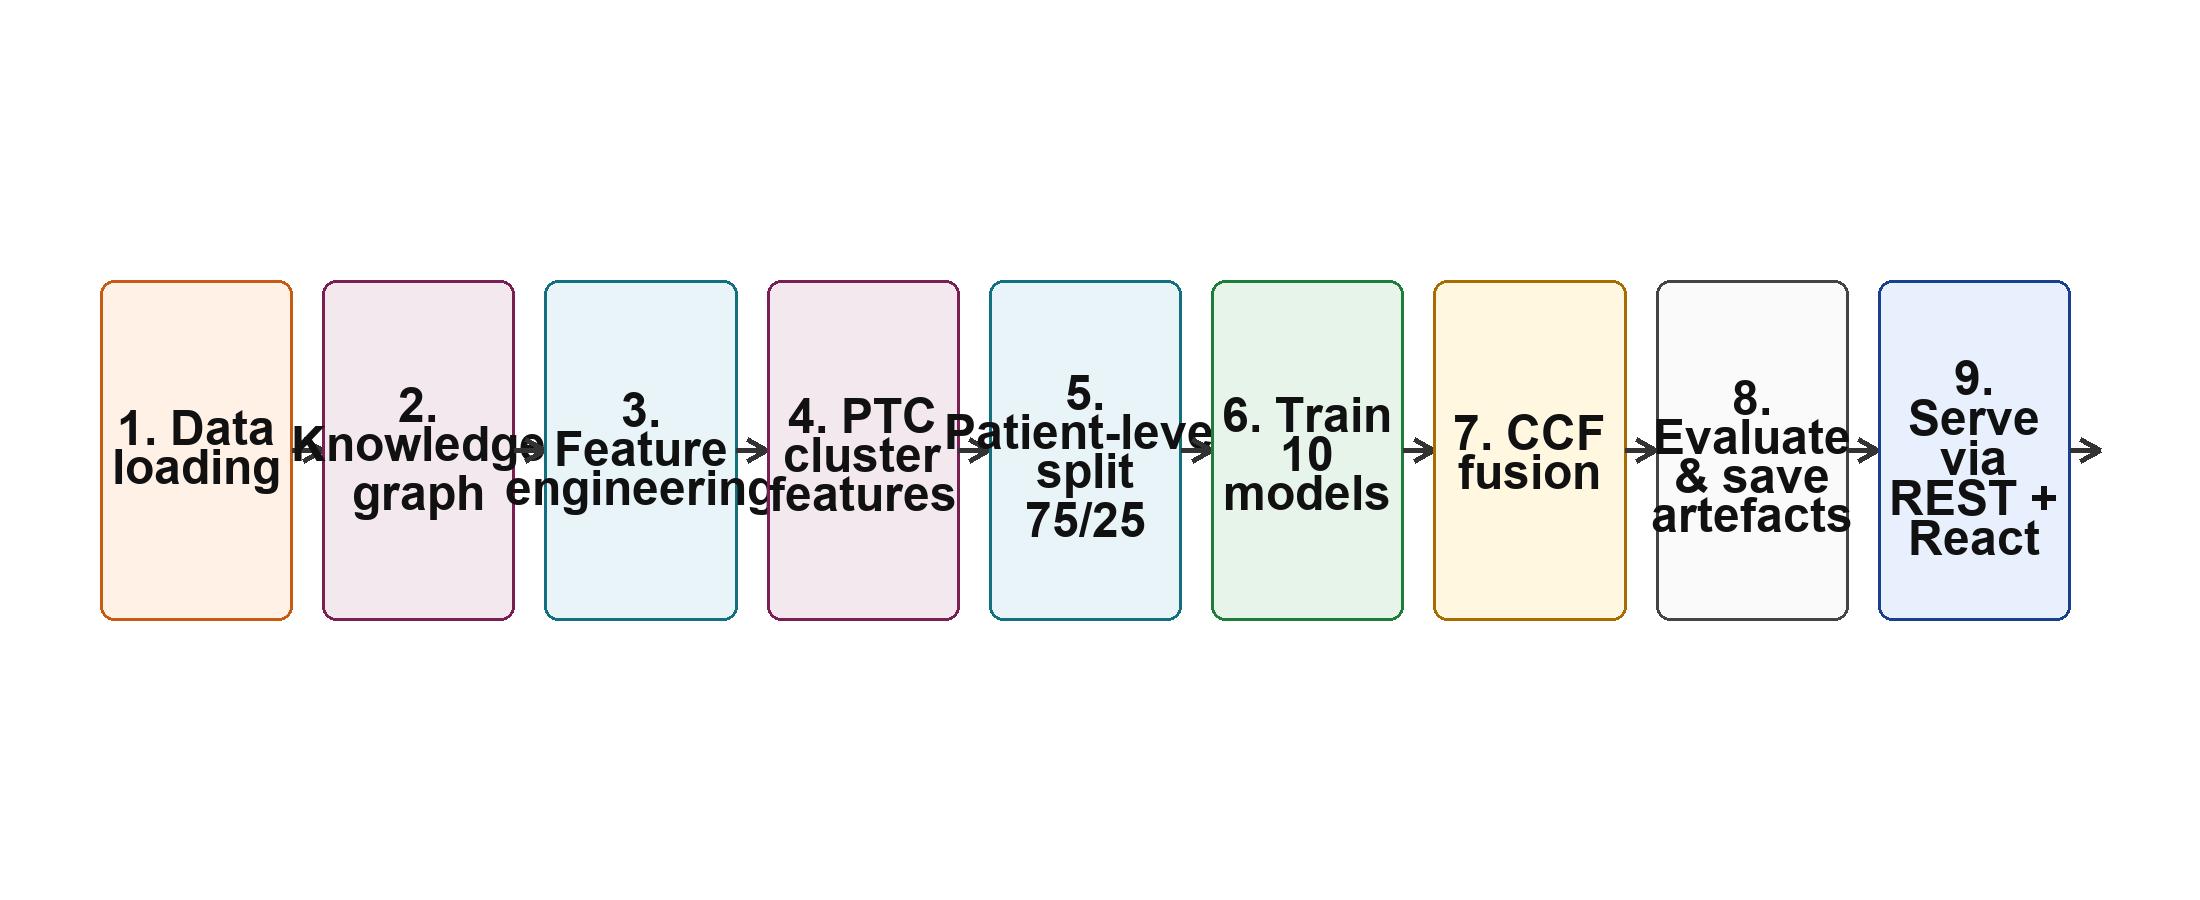
\includegraphics[width=\columnwidth]{figures/workflow.png}
\caption{End-to-end pipeline from data loading through evaluation and
serving.}
\label{fig:workflow}
\end{figure}

%----------------------------------------------------------------------
\section{Experiments and Results}

\subsection{Setup}

The synthetic cohort contains 240 patients and 960 visits (four visits
per patient). A patient-level stratified split retains 180 patients for
training and 60 for testing, so the evaluation reflects
\emph{generalisation to unseen patients} rather than unseen rows. All
metrics are computed on the test set with a 0.5 decision threshold.
Results for a final model run are summarised in
Table~\ref{tab:metrics}.

\subsection{Main Results}

\begin{table}[!t]
\caption{Patient-level test metrics over ten models. Best value in
each column in bold. AUC values are unavailable dimensions are omitted
(no degenerate splits occurred).}
\label{tab:metrics}
\centering
\small
\setlength{\tabcolsep}{2.4pt}
\renewcommand{\arraystretch}{1.05}
\begin{tabular}{lcccccccc}
\toprule
Model & Acc & Prec & Rec & F1 & ROC & PR & Brier & LL \\
\midrule
Logistic regression & 0.817 & 0.750 & 0.783 & 0.766 & 0.927 & 0.897 & 0.112 & 0.332 \\
Random forest       & 0.867 & 0.800 & 0.870 & 0.833 & 0.935 & 0.916 & 0.102 & 0.317 \\
XGBoost             & \textbf{0.900} & \textbf{0.870} & \textbf{0.870} & \textbf{0.870} & \textbf{0.955} & \textbf{0.945} & \textbf{0.082} & \textbf{0.261} \\
MLP                 & 0.817 & 0.731 & 0.826 & 0.776 & 0.910 & 0.851 & 0.143 & 0.757 \\
\midrule
GNN                 & 0.800 & 0.704 & 0.826 & 0.760 & 0.887 & 0.807 & 0.167 & 1.223 \\
GNN\,+\,KG          & 0.850 & 0.792 & 0.826 & 0.809 & 0.911 & 0.871 & 0.115 & 0.615 \\
GNN\,+\,KG\,+\,long.& 0.867 & 0.826 & 0.826 & 0.826 & 0.929 & 0.906 & 0.115 & 0.507 \\
\midrule
TAGNN               & 0.850 & 0.792 & 0.826 & 0.809 & 0.907 & 0.860 & 0.146 & 0.830 \\
MHFIN               & 0.850 & 0.792 & 0.826 & 0.809 & 0.911 & \textbf{0.899} & 0.154 & 1.070 \\
CCF fusion          & 0.867 & 0.800 & 0.870 & 0.833 & 0.931 & 0.916 & 0.119 & 0.406 \\
\bottomrule
\end{tabular}
\end{table}

Two findings stand out. First, the staged ablation over the graph
family confirms the value of each component: the plain GNN reaches
F1\,$=$\,0.760, adding knowledge-graph edges raises it to 0.809, and
adding longitudinal features raises it further to 0.826 (with ROC-AUC
improving from 0.887 to 0.929). Each architectural choice therefore
contributes a measurable, monotone improvement.

Second, the strong tabular baseline XGBoost posts the highest raw
scores in most columns, which is expected on a clean, fully specified
synthetic cohort: gradient boosting is a very strong learner on dense
tabular data. The value of the graph-based and fusion models lies in
where they are not worse in aggregate. CCF matches the best F1 of the
random forest (0.833) while substantially lowering log loss relative
to the individual neural and graph models (0.406 versus 0.507--1.223),
illustrating the effect of calibration on probability quality. Among
the novel methods, MHFIN attains the best PR-AUC (0.899) and ties the
knowledge-graph ROC-AUC (0.911) while remaining a purely tabular
model.

\subsection{Ablation and Interpretable Artefacts}

Table~\ref{tab:ablation} isolates the contributions of the three graph
stages across all metrics. The monotone improvement corroborates the
motivation of Section~\ref{sec:kg}: population knowledge and temporal
features each add predictive signal. The dashboard additionally exposes
an explanation probe for an exemplar test patient, the learned CCF
model coefficients, and per-node attention weights, keeping the
system's internal reasoning inspectable.

\begin{table}[!t]
\caption{Ablation over the three graph-model stages.}
\label{tab:ablation}
\centering
\small
\setlength{\tabcolsep}{2.4pt}
\renewcommand{\arraystretch}{1.05}
\begin{tabular}{lccccccccc}
\toprule
Stage & Acc & Prec & Rec & F1 & ROC & PR & Brier & LL \\
\midrule
gnn            & 0.800 & 0.704 & 0.826 & 0.760 & 0.887 & 0.807 & 0.167 & 1.223 \\
gnn\,+\,kg     & 0.850 & 0.792 & 0.826 & 0.809 & 0.911 & 0.871 & 0.115 & 0.615 \\
gnn\,+\,kg\,+\,long. & 0.867 & 0.826 & 0.826 & 0.826 & 0.929 & 0.906 & 0.115 & 0.507 \\
\bottomrule
\end{tabular}
\end{table}

%----------------------------------------------------------------------
\section{Serving Layer and Web Interface}

All pipeline outputs -- metric tables, ablation records, split
meta-data, trajectory clusters, CCF weights, explanation probes, and the
knowledge-graph file -- are consumed by a FastAPI backend. The API
exposes resource endpoints for metrics, ablation, split summary,
patients, dataset rows, explanations, clusters, fusion weights, the
knowledge graph, single-patient inference, and dataset ingestion. A
React dashboard built with Vite consumes these endpoints and
visualises the model comparison, the patient-level trajectory, the
interactive knowledge graph, feature explanations, clustering, ablation
comparison, and fusion weights. Fig.~\ref{fig:screenshot} shows the
model-comparison overview served by the deployed system.

\begin{figure}[!t]
\centering
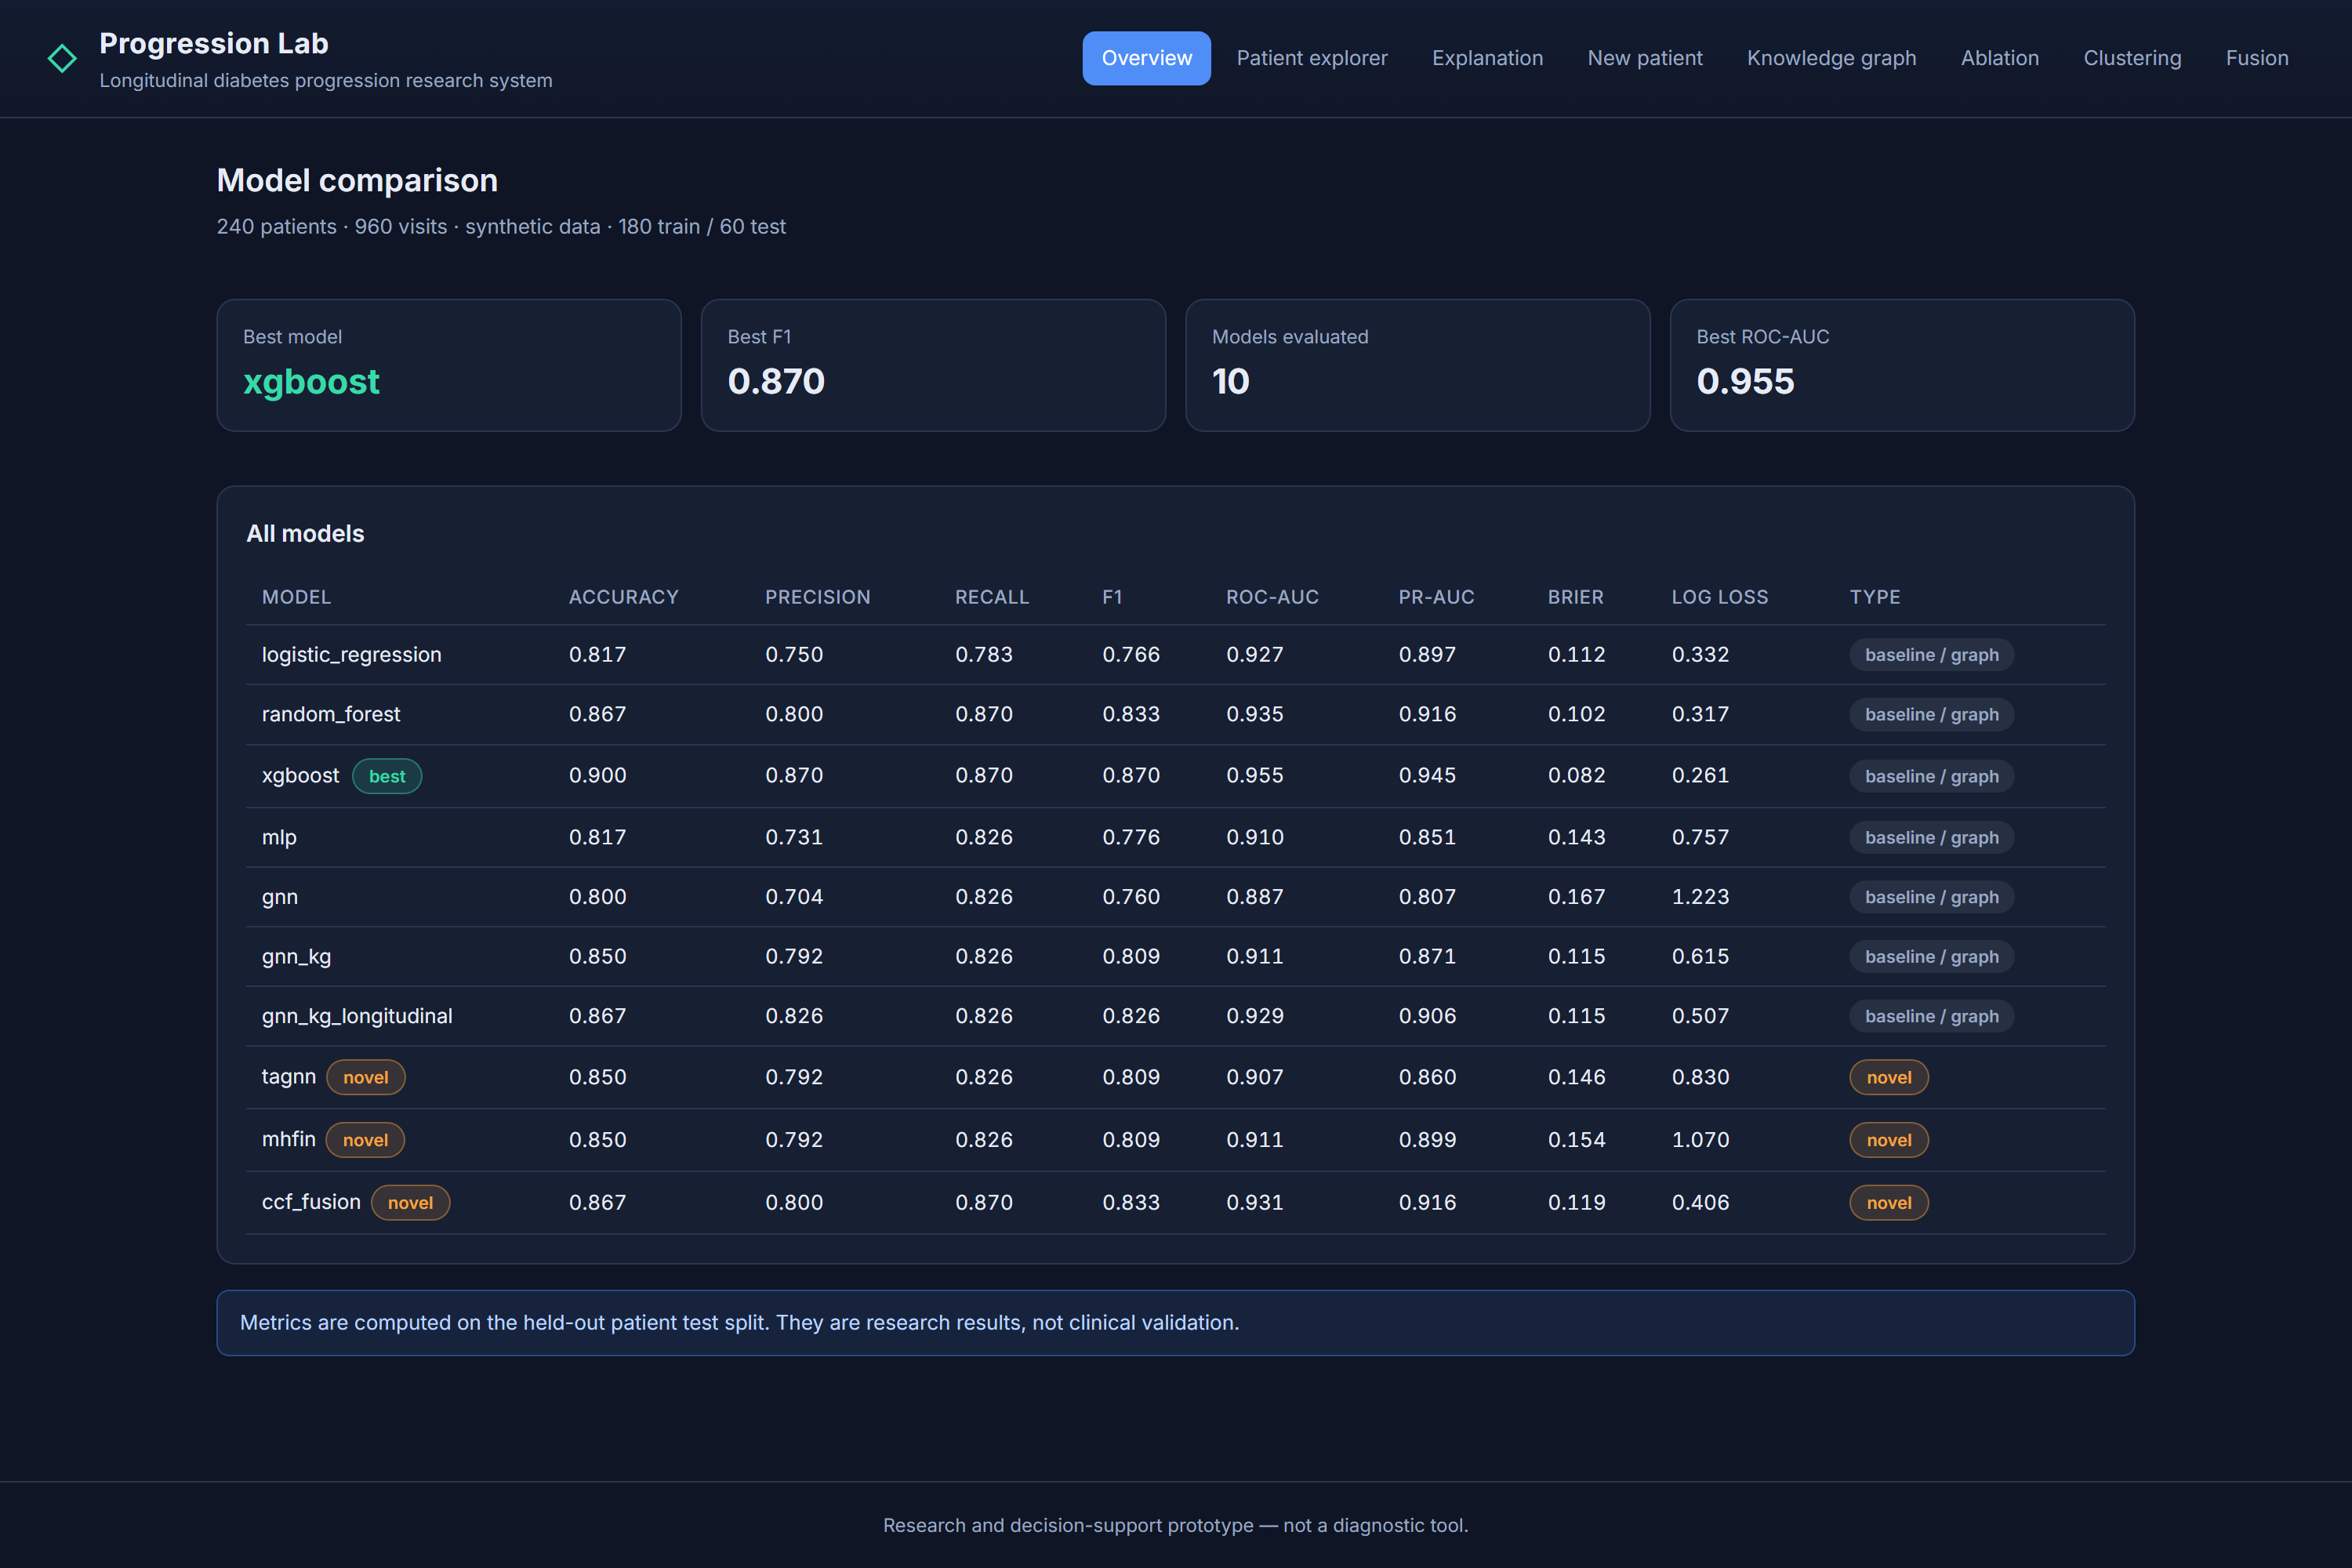
\includegraphics[width=\columnwidth]{figures/overview.png}
\caption{Model-comparison overview page. The best model, aggregate
statistics, and the ten-model metric table are rendered from the REST
endpoint.}
\label{fig:screenshot}
\end{figure}

%----------------------------------------------------------------------
\section{Discussion}

The results are best understood through three lenses. From a modelling
perspective, the ablation shows that relational structure and temporal
features are \emph{complementary} sources of signal in patient-level
prediction. From a practical perspective, the calibrated fusion
demonstrates that per-model reliability weighting can improve
probability quality without changing any base model. From a
deployment perspective, the layered architecture means each component
-- generator, graph builder, feature extractor, model, calibrator, or
visualisation -- can be replaced independently, which is valuable in a
research tool that must track evolving clinical endpoints.

It should be stressed that this is a research and decision-support
prototype. The synthetic cohort used for the headline numbers is
deliberately stylised, and no clinical claim is intended.

%----------------------------------------------------------------------
\section{Conclusion and Future Work}

We presented a complete longitudinal knowledge-graph-aware framework
for diabetes progression modelling, with four novel components --
TAGNN, MHFIN, CCF, and PTC -- embedded in a ten-model pipeline, a
patient-level evaluation protocol, and a live web serving layer. The
staged ablation demonstrates consistent gains from knowledge-graph
edges and longitudinal features, and calibrated fusion improves
probability quality over individual neural models.

Future work will validate the framework on the real Pima dataset and on
external longitudinal cohorts, benchmark TAGNN attention weights against
clinician-annotated progression signals, and extend CCF to asymmetric
loss weighting for screening applications where false negatives are
more costly than false positives.

\begin{thebibliography}{99}\scriptsize

\bibitem{ada} American Diabetes Association, ``Standards of care in
diabetes -- 2024,'' \emph{Diabetes Care}, vol.~47, suppl.~1, 2024.

\bibitem{scarselli} F.~Scarselli, M.~Gori, A.~C.~Tsoi,
M.~Hagenbuchner, and G.~Monfardini, ``The graph neural network model,''
\emph{IEEE Transactions on Neural Networks}, vol.~20, no.~1,
pp.~61--80, 2009.

\bibitem{kipf2017} T.~N.~Kipf and M.~Welling, ``Semi-supervised
classification with graph convolutional networks,'' in \emph{Proc.
International Conference on Learning Representations (ICLR)}, 2017.

\bibitem{hamilton2017} W.~L.~Hamilton, R.~Ying, and J.~Leskovec,
``Inductive representation learning on large graphs,'' in \emph{Proc.
Advances in Neural Information Processing Systems (NeurIPS)}, 2017.

\bibitem{vaswani} A.~Vaswani \etal, ``Attention is all you need,'' in
\emph{Proc. NeurIPS}, 2017, pp.~5998--6008.

\bibitem{guo} C.~Guo, G.~Pleiss, Y.~Sun, and K.~Q.~Weinberger, ``On
calibration of modern neural networks,'' in \emph{Proc. International
Conference on Machine Learning (ICML)}, 2017, pp.~1321--1330.

\bibitem{lime} M.~T.~Ribeiro, S.~Singh, and C.~Guestrin, ``Why should
I trust you? Explaining the predictions of any classifier,'' in
\emph{Proc. ACM SIGKDD}, 2016, pp.~1135--1144.

\bibitem{shap} S.~M.~Lundberg and S.-I. Lee, ``A unified approach to
interpreting model predictions,'' in \emph{Proc. NeurIPS}, 2017,
pp.~4765--4774.

\bibitem{breiman} L.~Breiman, ``Random forests,'' \emph{Machine
Learning}, vol.~45, no.~1, pp.~5--32, 2001.

\bibitem{xgboost} T.~Chen and C.~Guestrin, ``XGBoost: A scalable tree
boosting system,'' in \emph{Proc. ACM SIGKDD}, 2016, pp.~785--794.

\bibitem{pima} J.~W.~Smith, J.~E.~Everhart, W.~C.~Dickson, W.~C.
Knowler, and R.~S.~Johannes, ``Using the ADAP learning algorithm to
forecast the onset of diabetes mellitus,'' in \emph{Proc. Symposium on
Computer Applications and Medical Care}, 1988, pp.~261--265.

\end{thebibliography}

\end{document}